\documentclass{article}
\usepackage[preprint, nonatbib]{neurips_2020}

\usepackage[utf8]{inputenc}
\usepackage[T1]{fontenc}
\usepackage{amsfonts}
\usepackage{microtype}
\usepackage{hyperref}

\usepackage{booktabs}
\usepackage{graphicx}
\usepackage[square,numbers]{natbib}
\usepackage{makecell}
\usepackage[ruled,vlined]{algorithm2e}
\usepackage{subcaption}
\usepackage{textcomp}

\title{Supplementary material for MeLES: Metric learning for event sequences with self-supervision}

\author{
Dmitrii Babaev\thanks{D. Babaev N. Ovsov and I. Kireev contributed equally to this work.} \\
% dmitri.babaev@gmail.com
Sberbank AI Lab
\And
Ivan Kireev \\
Sberbank AI Lab
\And
Nikita Ovsov \\
Sberbank AI Lab
\And
Maria Ivanova \\
Sberbank AI Lab
\And
Gleb Gusev \\
Sberbank AI Lab
\And
Alexander Tuzhilin \\
% \email{atuzhili@stern.nyu.edu}
New York University
}

\begin{document}

\maketitle

\section{Experiments} \label{sec-exp}

\section{Datasets}



We designed the method specially for the user behavior sequences~\cite{Ni2018PerceiveYU}. That sequences consist of discrete events per person in continuous time, for example,  behavior on websites, credit card transactions, etc. 

Considering credit card transactions, each transaction have a set of attributes, either categorical or numerical including the timestamp of the transaction. An example of the sequence of three transactions with their attributes is presented in the Table \ref{tab-tr-data}.
Merchant type field represents the category of a merchant, such as "airline", "hotel", "restaurant", etc.

\begin{table}
\centering
\caption{Data structure for a single credit card}
\begin{tabular}{llllll}
\toprule
\textbf{Date} & \textbf{Time} & \textbf{Amount} & \textbf{Currency} & \textbf{Country} & \textbf{Merchant Type} \\
\midrule
Jun 21 & 16:40& 230 & EUR & France & Restaurant \\
Jun 21 & 20:15 & 5 & USD & US & Transportation \\
Jun 22 & 09:30 & 40 & USD & US & Household Appliance \\
\bottomrule
\end{tabular}
\label{tab-tr-data}
\end{table}

Another example of user behavior data is click-stream: the log of internet pages  visits. The example of a click-stream log of a single user is presented in Table \ref{tab-cs-data}.

\begin{table}
\centering
\caption{Click-stream structure for a single user}
\begin{tabular}{llll}
\toprule
\textbf{Time} & \textbf{Date} & \textbf{Domain} & \textbf{Referrer Domain} \\
\midrule
17:40 & Jun 21 & amazon.com & google.com \\
17:41 & Jun 21 & amazon.com & amazon.com \\
17:45 & Jun 21 & en.wikipedia.org & google.com \\
\bottomrule
\end{tabular}
\label{tab-cs-data}
\end{table}


In our research we used several publicly available datasets of bank transactions.
\begin{enumerate}
    \item \textbf{Age group prediction competition}\footnote{https://onti.ai-academy.ru/competition} - the task is to predict the age group of a person. The dataset consists of 44M anonymized transactions representing 50k persons with a target labeled for only 30k of them (27M out of 44M transactions), for the other 20k persons (17M out of 44M transactions) label is unknown. Each transaction includes date, type (for example, grocery store, clothes, gas station, children's goods, etc.) and amount. We use all available 44M transactions for metric learning, excluding 10\% - for the test part of the dataset, and  5\% for the metric learning validation.
        
    \item \textbf{Prediction of client gender on card transactions}\footnote{https://www.kaggle.com/c/python-and-analyze-data-final-project/} - the task is a classification problem of predicting a gender. The dataset consists of 6,8M anonymized card transactions representing 15k clients, where only 8,4k of them are labeled. Each transaction is characterized by date, type (for ex. "ATM cash deposit"), amount and Merchant Category Code (MCC).
    
    \item \textbf{Data Science Bowl}\footnote{https://www.kaggle.com/c/data-science-bowl-2019} - the task is to predict the in-game assessments results based on the history of children gameplay data. The dataset consists of 12M gameplay events representing 4,6k children. Each gameplay event is characterized by timestamp, event code, incremental counter of events within a game session, time since the start of the game session, etc.
    
    \item \textbf{Gender prediction competition}\footnote{https://ods.ai/competitions/x5-retailhero-uplift-modeling} - the task is to predict the age group of a client based on it retail purchase history. The dataset consists of ???M retail purchases representing ???k clients. Each purchase is characterized by time, product level, segment, amount, value, points received.
    
    
    
    
\end{enumerate}


\subsection{Experiment setup}

\begin{table}
\centering
\caption{Hyper-parameters for MeLES training}
\begin{tabular}{lllll}
\toprule
\textbf{Dataset} & \textbf{Learning rate} & \textbf{N samples in batch} & \textbf{N epochs} & \textbf{N sub-samples} \\
\midrule
\textbf{Age group} & 0.002 & 64 & 100 & 5 \\
\textbf{Gender} & 0.002 & 128 & 150 & 5 \\
\bottomrule
\end{tabular}
\label{tab-hyper}
\end{table}

\subsection{Baselines} \label{sec-baselines}

Here we describe the the details of producing hand-crafted features. All attributes of each transaction are either numerical (e. g. amount) or categorical (e.g. merchant type (mcc code), transaction type, etc.). 
For numerical type of attribute we apply aggregation functions, such as 'sum', 'mean', 'std', 'min', 'max', over all transactions per user. For example, if we apply 'sum' for the numerical field 'amount' we obtain a feature 'sum of all transaction amounts per user'. 
For categorical type of attribute we apply aggregation functions in a slightly different way. For each unique value of categorical attribute we apply aggregation functions, such as 'count', 'mean', 'std' over all transactions per user' numerical attribute. For example, if we apply 'mean' for the numerical attribute 'amount' grouped by categorical attribute 'mcc code' we obtain a feature 'mean amount of all transaction for each mcc code per user'. 
For example, for age prediction task we have one categorical attribute (small group) with 200 unique values, combining it with amount we can produce $200 * 3$ features ('group0 x amount x count',  'group1 x amount x count', ..., 'group199 x amount x count', 'group0 x amount x mean', ...). In total we use approx 605 features for age prediction task. For gender prediction task we have two categorical features: 'mcc code' with approx 200 unique values and 'tr type' with approx 100 unique values. So in total we use $200 * 3 + 100 * 3 + 5 = 905$ features.
Note, that hand-crafted features contain information about user spending profile but omit information about transactions temporal order.

\subsection{Design choices}

In the Table \ref{tab-enc-type} and Table \ref{tab-loss-type} we present the results of experiments on different design choices of our method.

As shown in Table \ref{tab-enc-type}, different choices of encoder architectures show comparable performance on the downstream tasks.

It is interesting to observe that even contrastive loss that can be considered as the basic variant of metric learning loss allows to get strong results on the downstream tasks (see Table \ref{tab-loss-type}). Our hypothesis is that an increase in the model performance on metric learning task does not always lead to an increase in performance on downstream tasks.

\begin{table}
\centering
\caption{Comparison of encoder types}
\begin{tabular}{llll}
\toprule
\textbf{Dataset} & \textbf{LSTM} & \textbf{GRU} & \textbf{Transformer} \\
\midrule
\textbf{Age group} \small{(Accuracy)} & 0.620 $\pm 0.003$ & $0.639 \pm 0.006$ & $0.621 \pm 0.001$ \\
\textbf{Gender} \small{(AUROC)} & $0.870 \pm 0.005$ & $0.871 \pm 0.004$ & $0.848 \pm 0.002$  \\
\bottomrule
\end{tabular} \\
\small{5-fold cross-validation metric $\pm 95\%$ is shown}
\label{tab-enc-type}
\end{table}

\begin{table}
\centering
\caption{Comparison of metric learning losses}
\begin{tabular}{llllll}
\toprule
\textbf{Dataset} & \textbf{Contrastive} & \makecell{\textbf{Binomial} \\ \textbf{deviance}} & \textbf{Histogram} & \textbf{Margin} & \textbf{Triplet} \\
\midrule
\makecell{\textbf{Age group} \\ \small{(Accuracy)}} & \makecell{0.639 \\ $\pm 0.006$} & \makecell{0.535 \\ $\pm 0.005$} & \makecell{0.642 \\ $\pm 0.002$} & \makecell{0.631 \\ $\pm 0.003$} & \makecell{0.610 \\ $\pm 0.006$} \\
\makecell{\textbf{Gender} \\ \small{(AUROC)}} & \makecell{0.871 \\ $\pm 0.003$} & \makecell{0.853 \\ $\pm 0.005$} & \makecell{0.851 \\ $\pm 0.004$} & \makecell{0.871 \\ $\pm 0.004$} & \makecell{0.855 \\ $\pm 0.003$} \\
\bottomrule
\end{tabular} \\
\small{5-fold cross-validation metric $\pm 95\%$ is shown}
\label{tab-loss-type}
\end{table}

\begin{figure}
  \centering
  \caption{Embedding dimensionality vs. quality}
  \begin{subfigure}{0.5\linewidth}
    \caption{Age group prediction}
    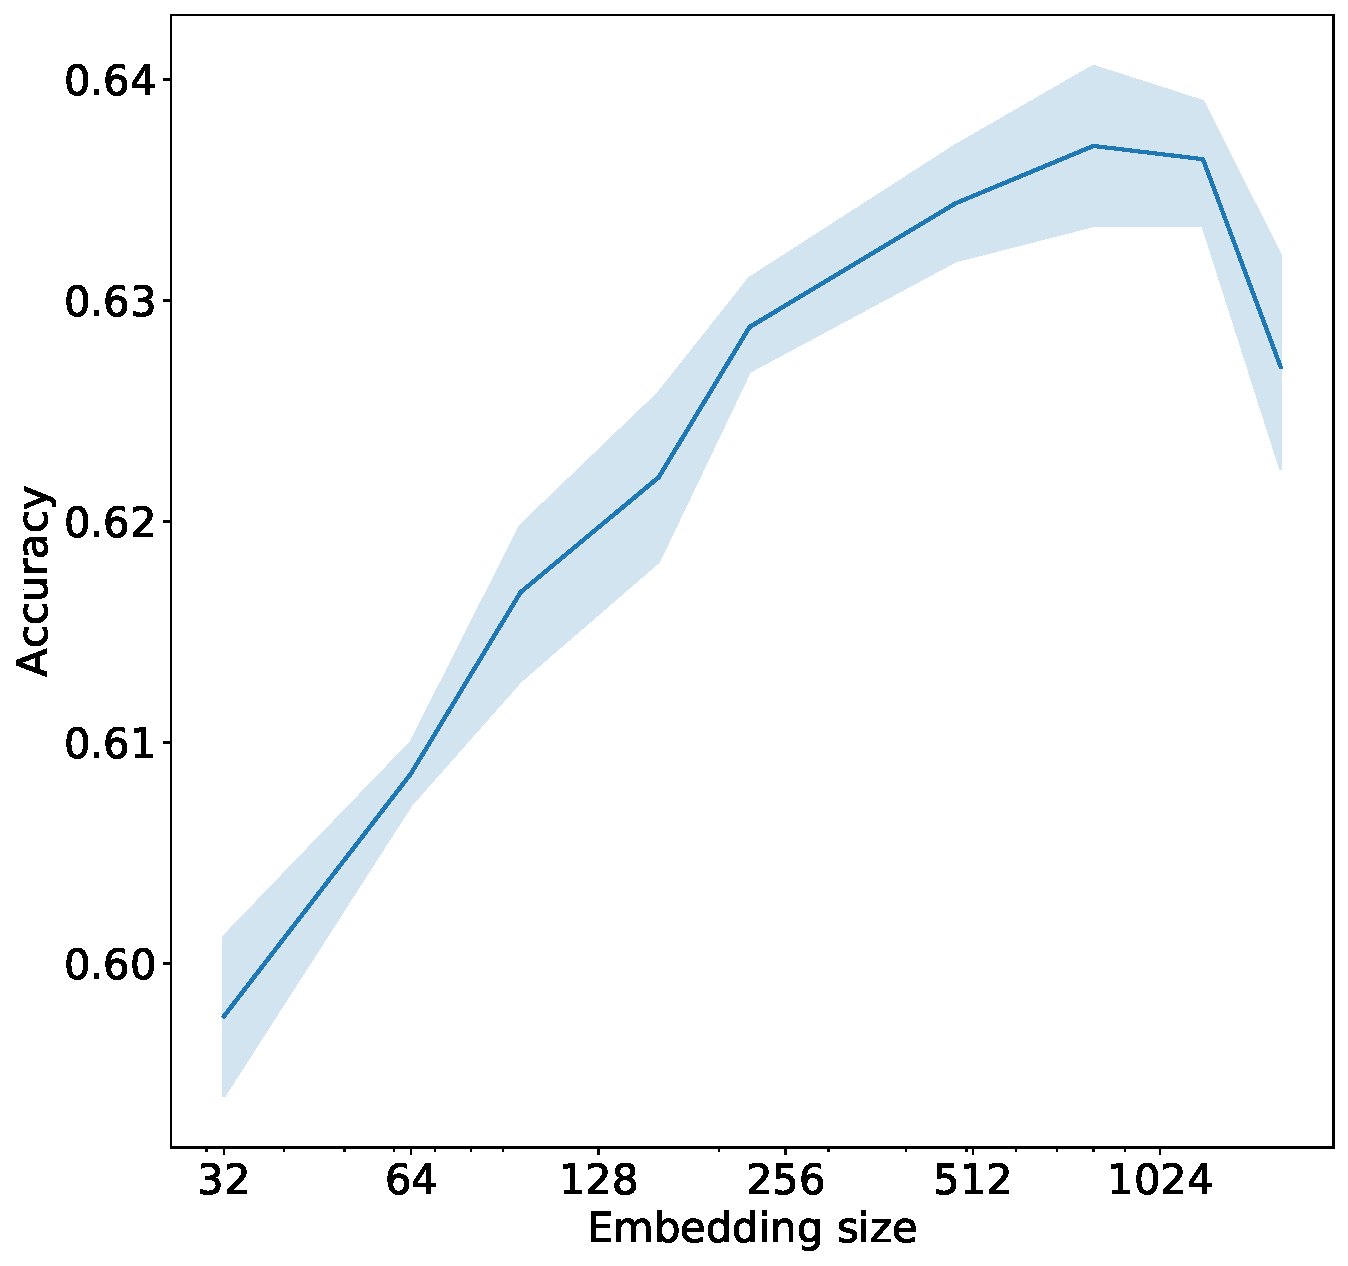
\includegraphics[width=\linewidth]{figures/age-pred-hidden-size.pdf}
    \label{fig-emb-dim-age}
  \end{subfigure}%
  \begin{subfigure}{0.5\linewidth}
    \caption{Gender prediction}
    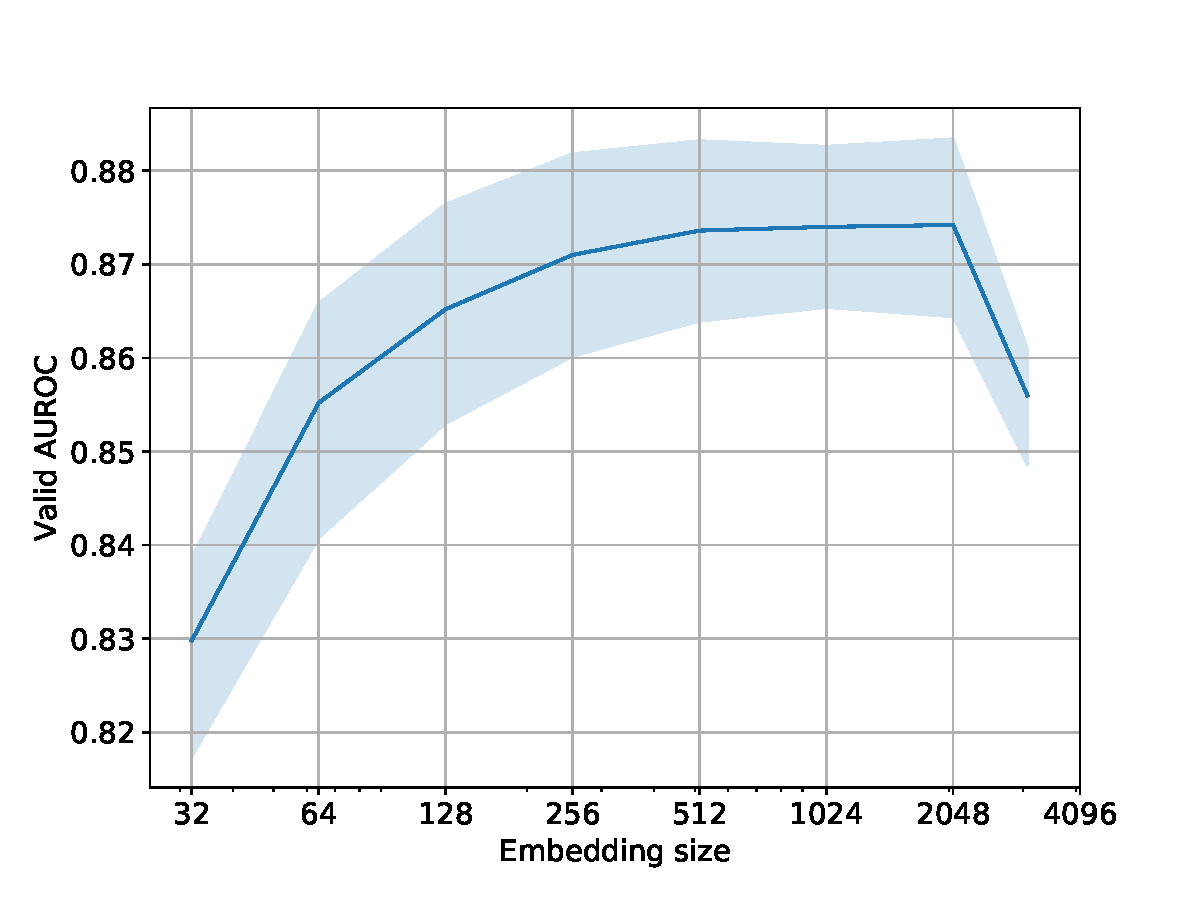
\includegraphics[width=\linewidth]{figures/gender-hidden-size.pdf}
    \label{fig-emb-dim-gender}
  \end{subfigure}
\end{figure}

\section{Results}

\subsection{Semi-supervised setup}

\begin{figure}
  \centering
  \begin{subfigure}{0.5\linewidth}
    \caption{Age group prediction}
    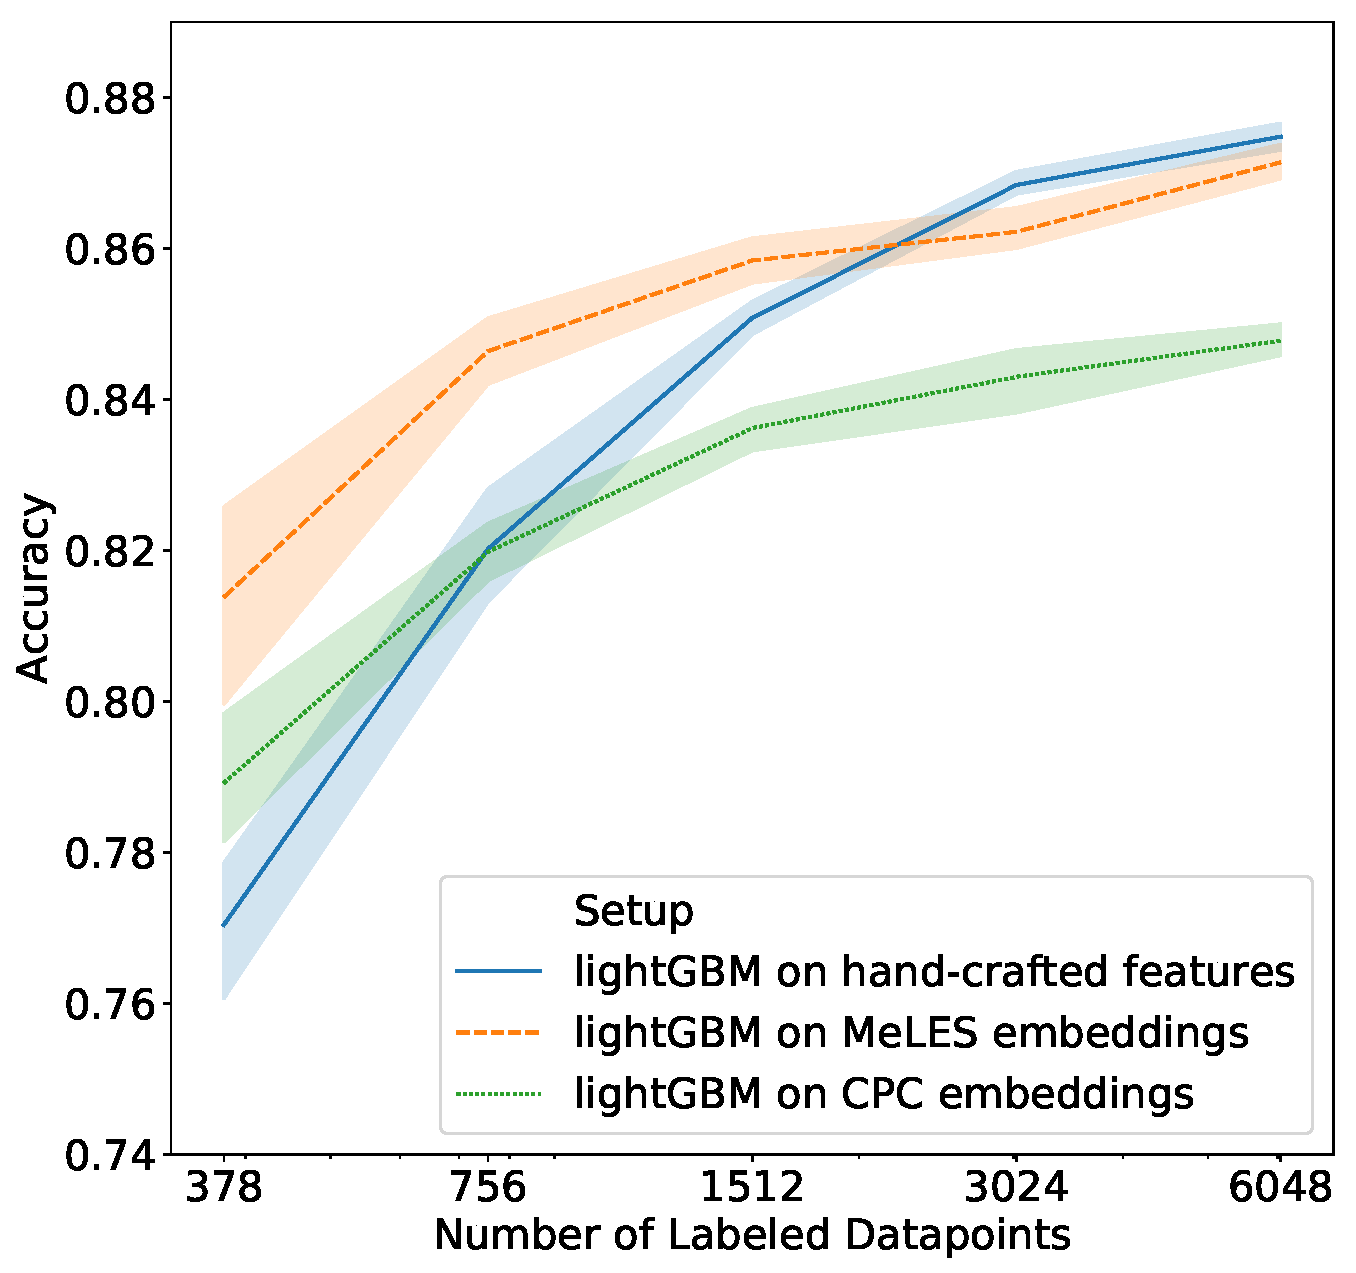
\includegraphics[width=\linewidth]{figures/ss_age_0.pdf}
    \label{fig-semi-age-0}
  \end{subfigure}%
  \begin{subfigure}{0.5\linewidth}
    \caption{Gender prediction}
    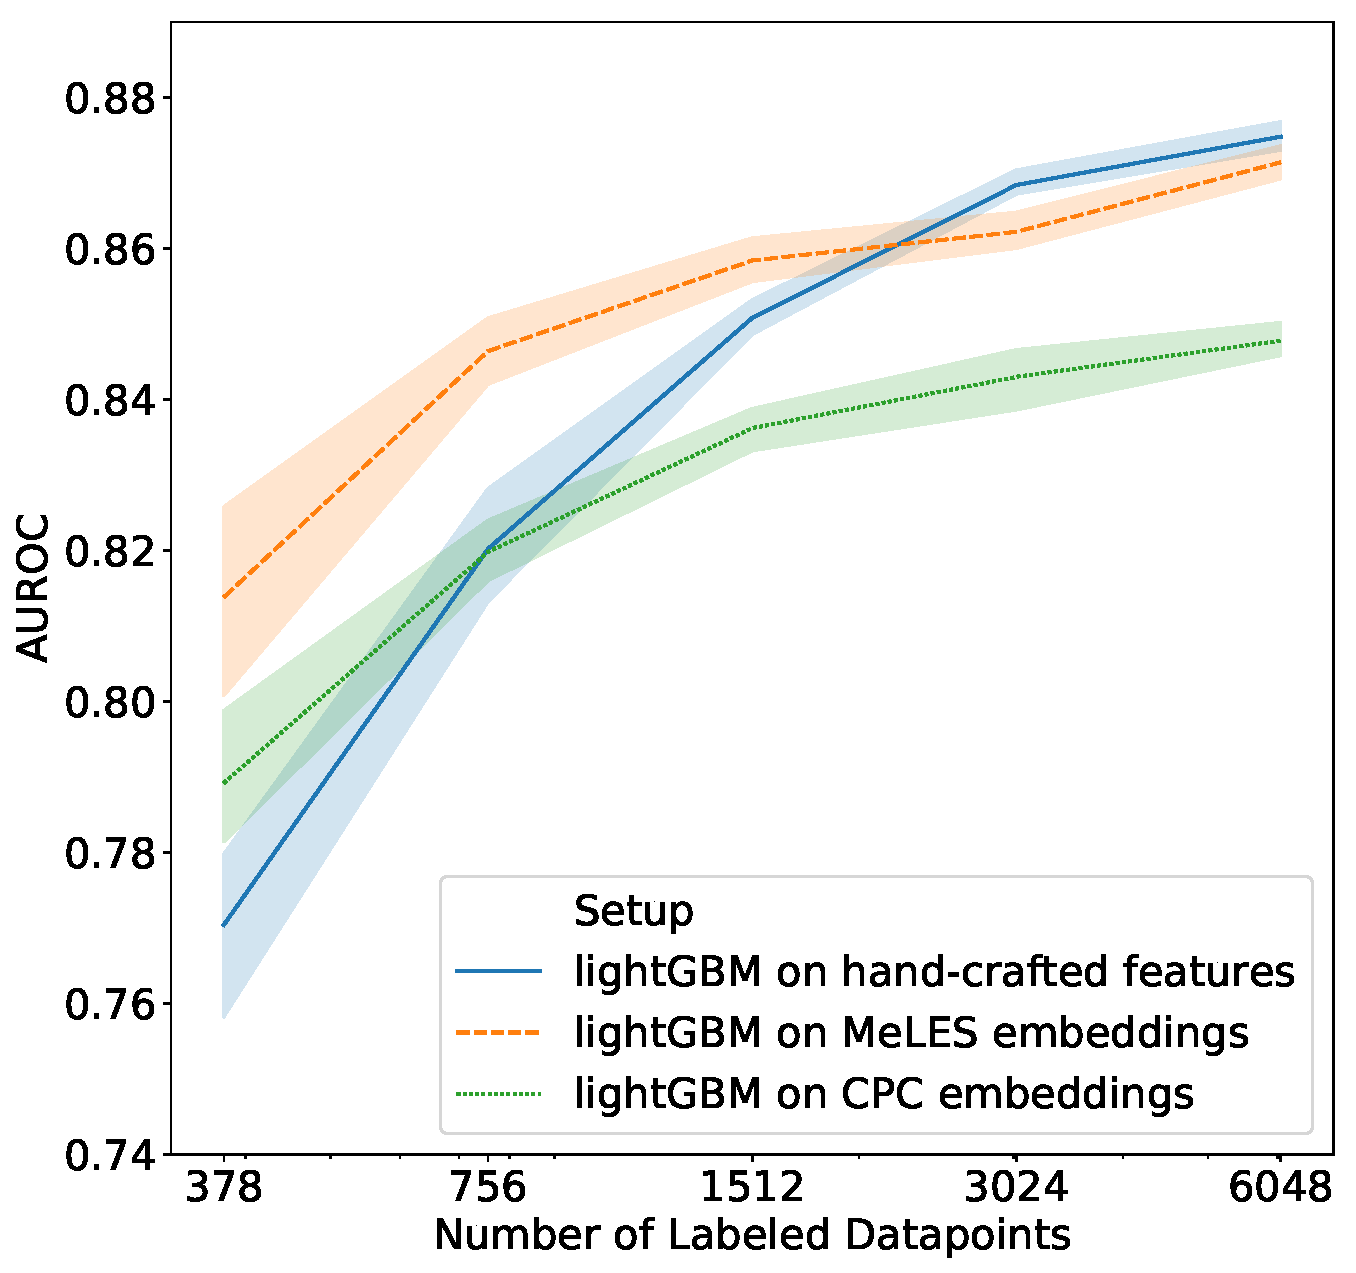
\includegraphics[width=\linewidth]{figures/ss_gen_0.pdf}
    \label{fig-semi-gender-0}
  \end{subfigure}
  \begin{subfigure}{0.5\linewidth}
    \caption{Age group prediction}
    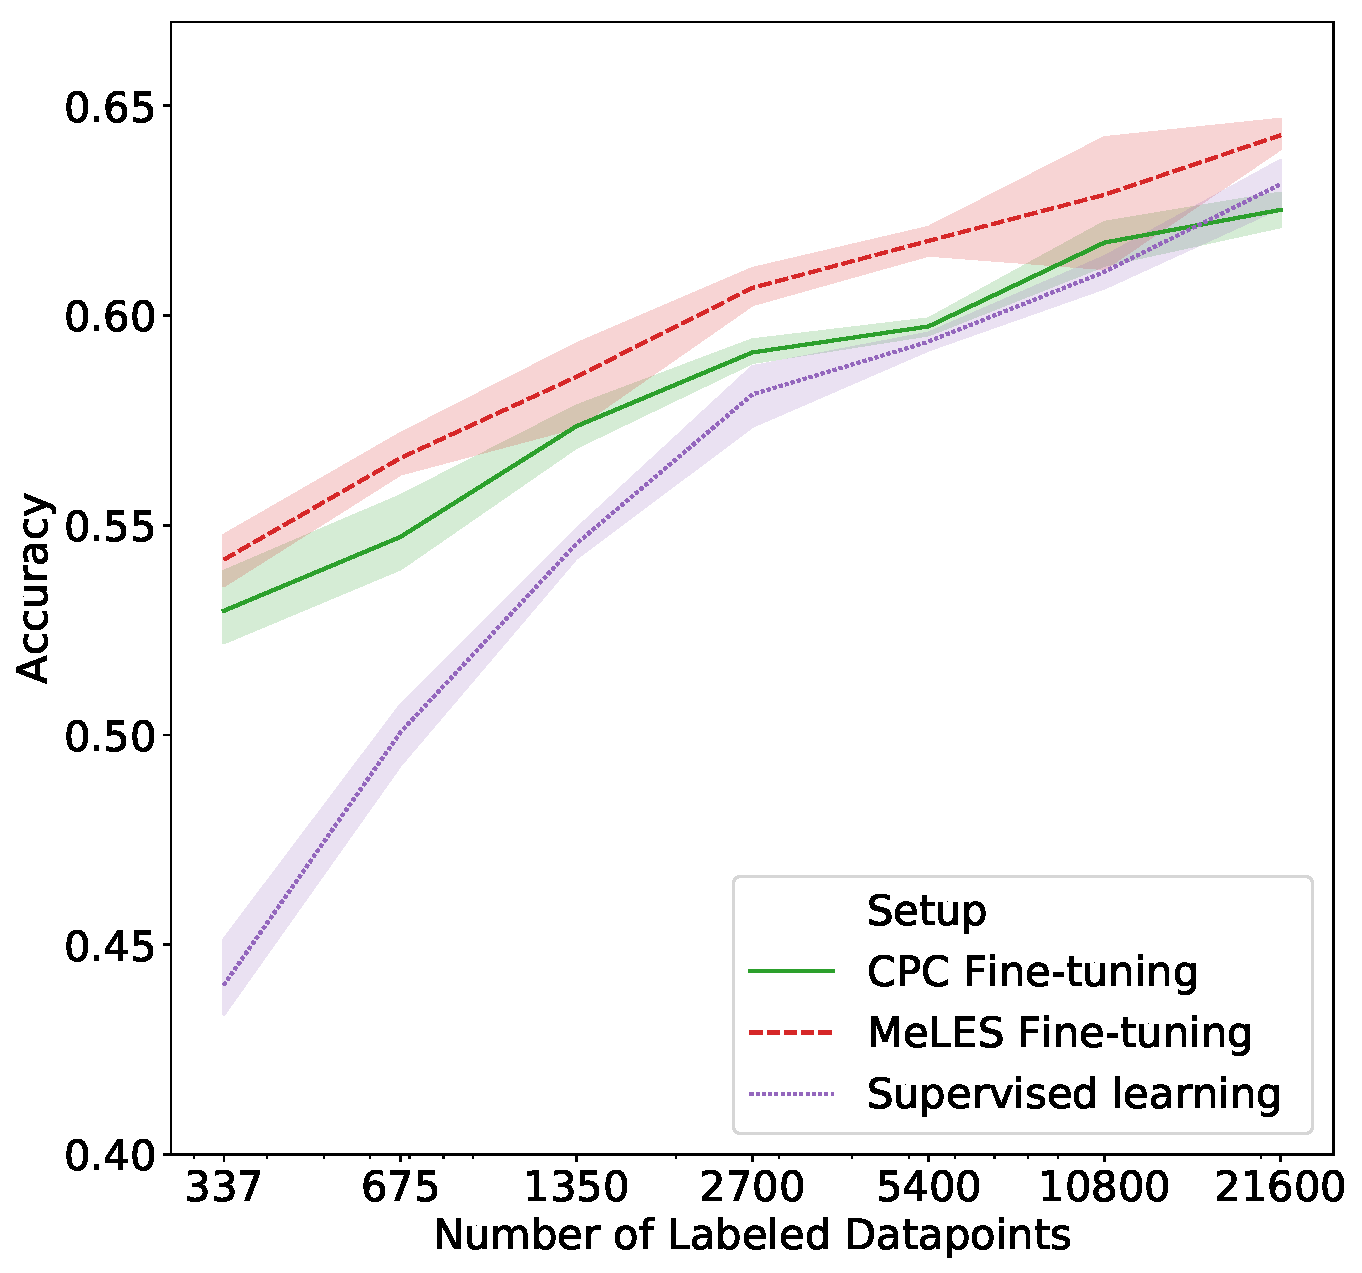
\includegraphics[width=\linewidth]{figures/ss_age_1_wopl.pdf}
    \label{fig-semi-age-1}
  \end{subfigure}%
  \begin{subfigure}{0.5\linewidth}
    \caption{Gender prediction}
    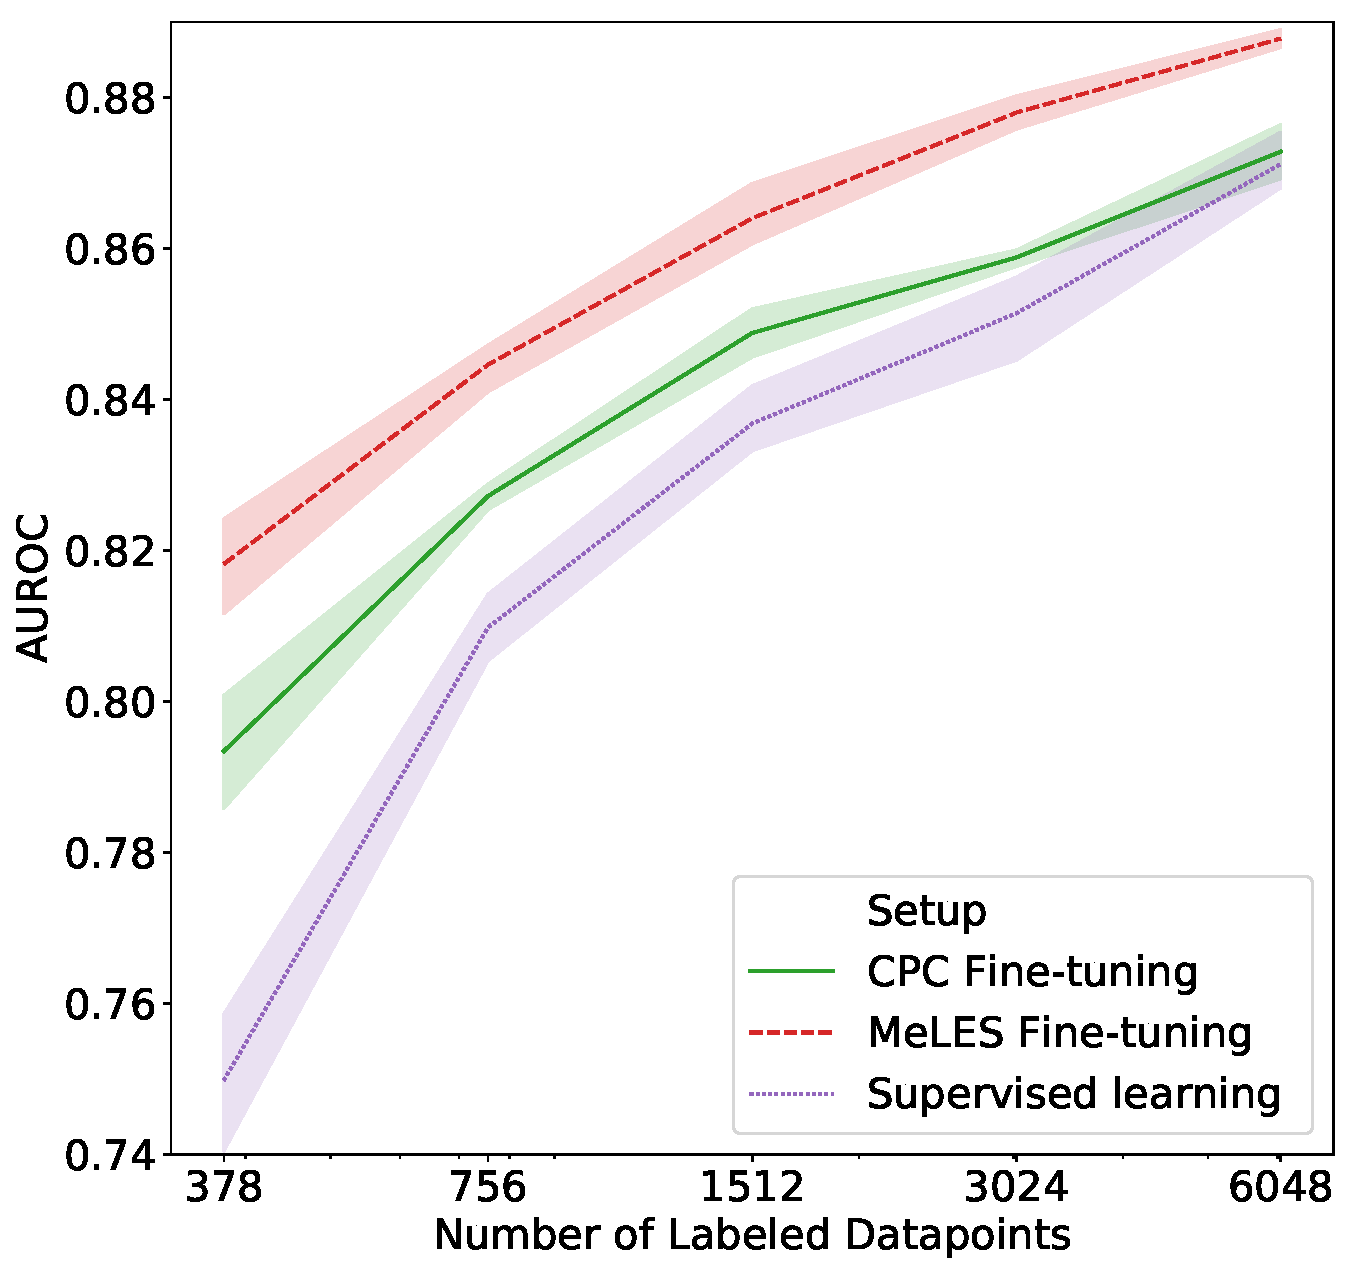
\includegraphics[width=\linewidth]{figures/ss_gen_1.pdf}
    \label{fig-semi-gender-1}
  \end{subfigure}
  \caption{Model quality for different dataset sizes} \small{The rightmost point correspond to all labels and supervised setup. X-axis is shown on a logarithmic scale.}
\end{figure}

\subsection{Embedding visualization}

In order to visualize MeLES embeddings in 2-dimensional space, we applied tSNE transformation~\cite{Maaten2008VisualizingDU} on them. tSNE transforms high-dimensional space to low-dimensional based on local relationships between points, so neighbour vectors in high-dimensional embedding space are pushed to be close in 2-dimensional space. We colorized 2-dimensional vectors using the target values of the datasets.

Note, that embeddings was learned in a fully self-supervised way from raw user transactions without any target information. Sequence of transactions represent user' behavior, thus the MeLES model captures behavioral patterns and outputs embeddings of users with similar patterns nearby.
As shown below, local clusters in embedding space correspond to distribution of user's attributes either age or gender.

tSNE vectors from the age prediction dataset are presented in the Figure \ref{fig-tsne-age}. We can observe 4 clusters: clusters for group '1' and '2' are on the opposite side of the cloud, clusters for groups '2' and '3' are in the middle.

Taking into account that age is an ordinal attribute, we can make an assumption about the ordering of age groups: $age(1) < age(3) < age(0) < age(2)$ or vice versa. ($age(bin)$ returns age of user for specific group).

tSNE points from gender prediction dataset are presented in the Figure \ref{fig-tsne-gender}. There are areas dominated by one gender label over another.

\begin{figure}
  \centering
  \caption{2D tSNE mapping of MeLES embeddings colored by target labels}
  \begin{subfigure}{0.5\textwidth}
    \caption{Age prediction dataset}
    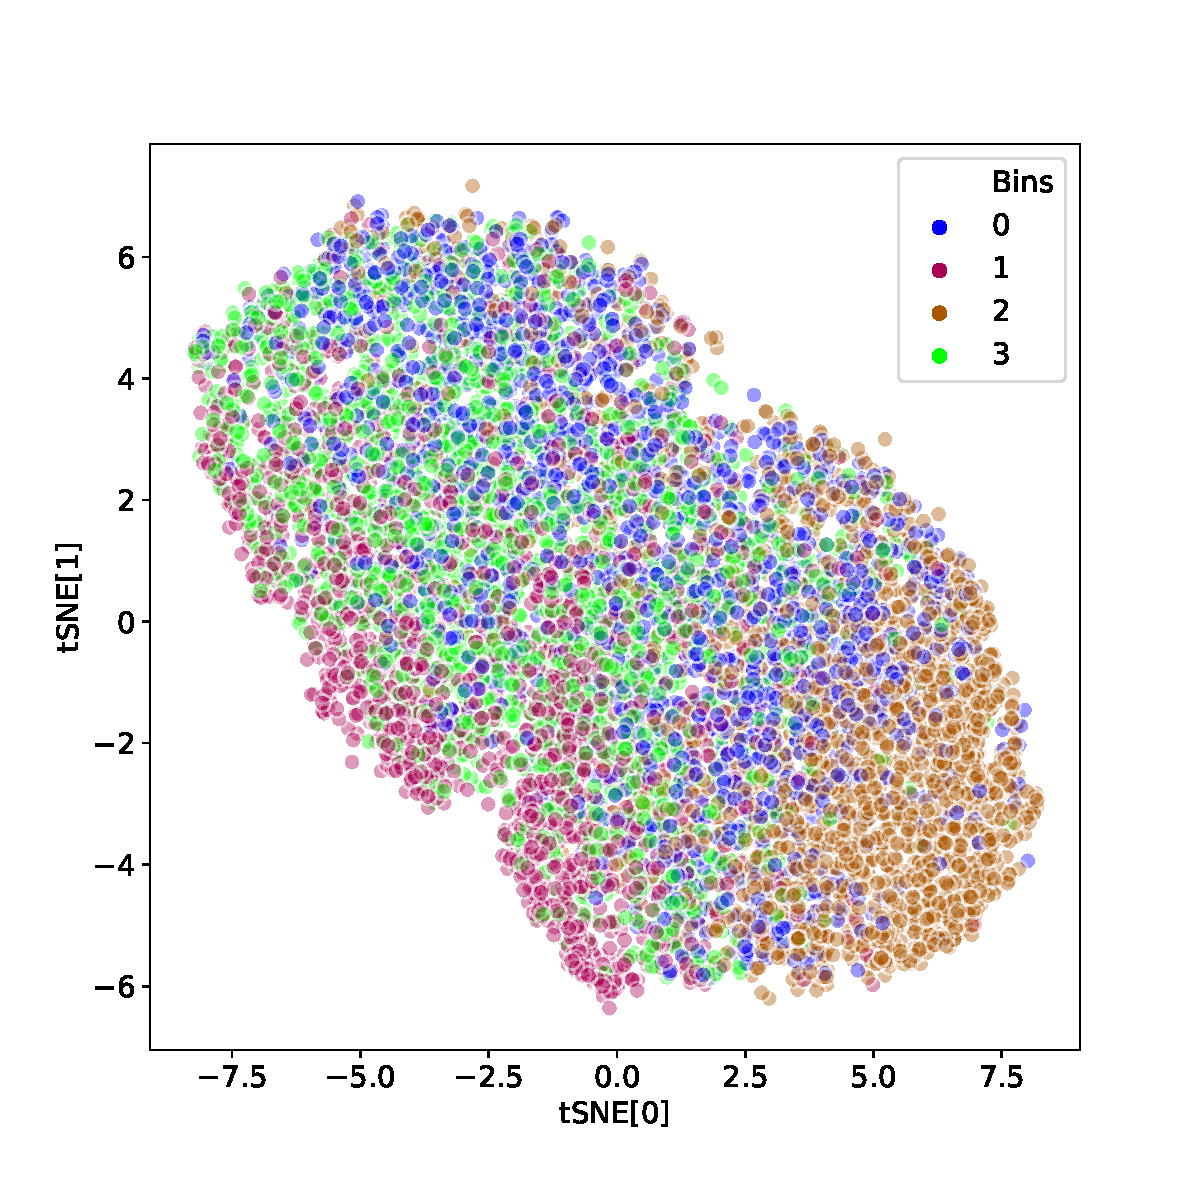
\includegraphics[width=\textwidth]{figures/age-pred-tsne.pdf}
    \label{fig-tsne-age}
  \end{subfigure}%
  \begin{subfigure}{0.5\textwidth}
    \caption{Gender prediction dataset}
    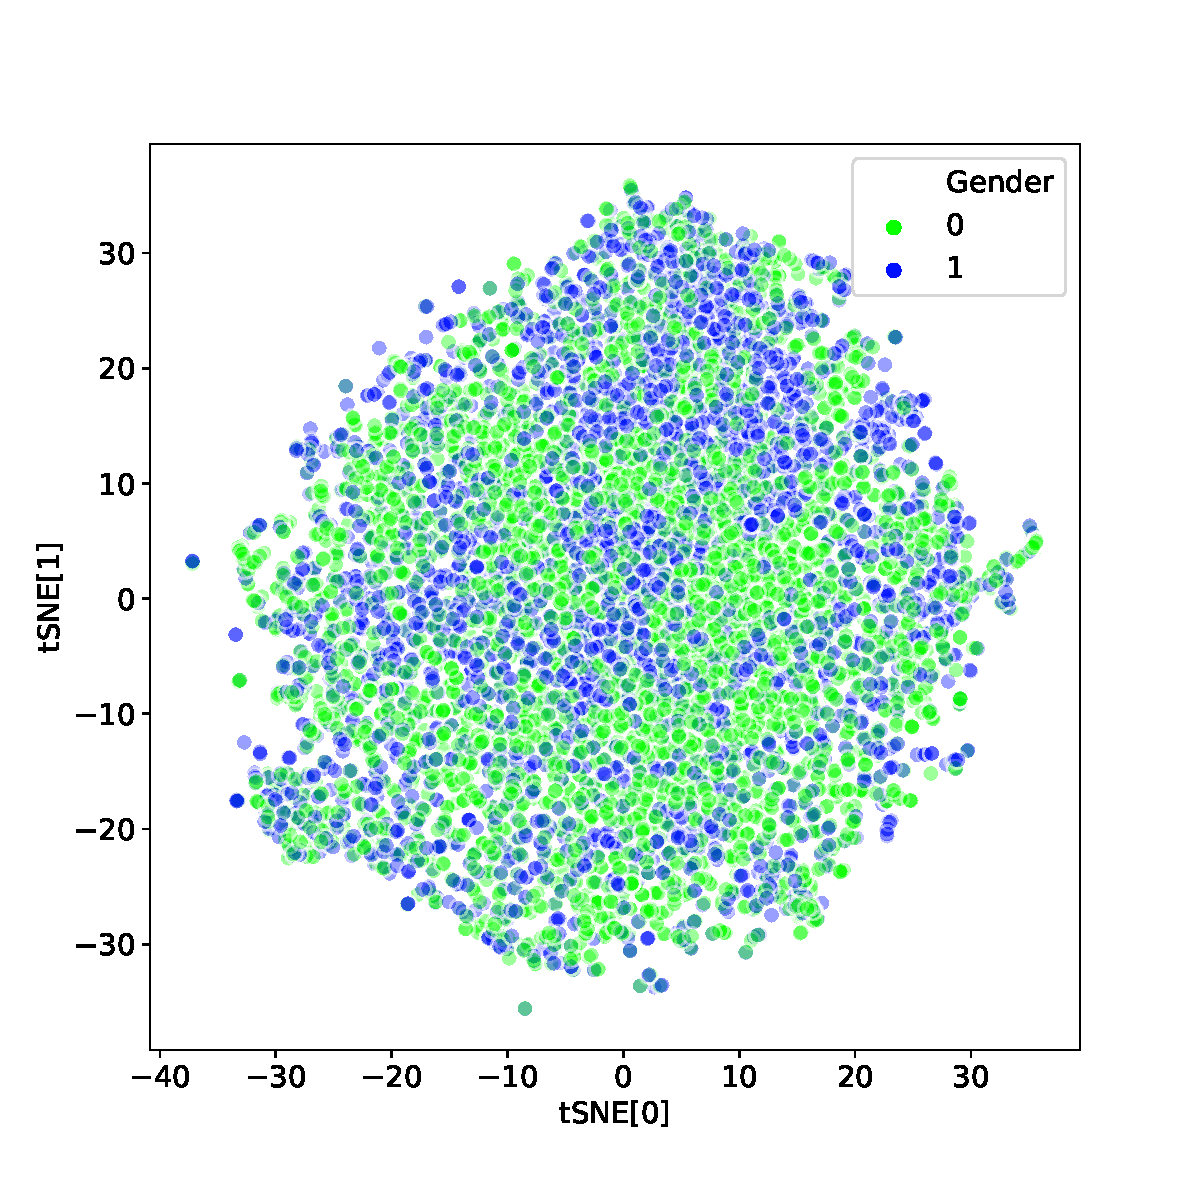
\includegraphics[width=\textwidth]{figures/gender-tsne.pdf}
    \label{fig-tsne-gender}
  \end{subfigure}
\end{figure}

\bibliographystyle{humannat}
\bibliography{neurips2020}

\end{document}